\chapter{Model Extensions}\label{chpt:Model_Extensions}
The prime objective of this chapter is to extend the event-driven model of Chapter \ref{chpt:ED} in two different ways. On one hand, in Section \ref{sec:GBM} the risky asset will be modeled in continuous-time as a \gls{GBM}, on the other hand, in Section \ref{sec:Interest_rate_dynamics} we no longer let the risk-free asset evolve deterministically but instead its short-rate will evolve according to the Vasicek model. 
\section{A GBM dynamics for the risky asset}\label{sec:GBM}
Let us consider the same portfolio as the one in Chapter \ref{chpt:ED}, namely a risky and a risk-free asset. As far as the risk-free asset is concerned, the deterministic model of Chapter \ref{chpt:ED} remains unchanged. On the other hand, the following dynamics for the risky asset is assumed
\begin{equation}\label{eq:GBM_SDE}
\begin{cases*}
dS_t  = \mu S_t dt + \sigma S_t dW_t\\
S_{t_k} = S_k, \quad t\geq t_k
\end{cases*}
\end{equation}
where $\{W_t\}_{t\geq t_k}$ is a unidimensional Brownian motion, $\mu \in \mathbb{R}$, $\sigma > 0$ and $t_k$ is the time when the $k$th event occurs. Solving the above \gls{SDE} brings 
\begin{align*}
S_t & = S_k \exp\big\{(\mu-\sigma^2/2)(t-t_k)+\sigma(W_t-W_{t_k})\}\\
& = S_k \exp\big\{\widetilde{\mu}(t-t_k)+\sigma(W_t-W_{t_k})\}
\end{align*}
where we defined $\widetilde{\mu}= \mu-\sigma^2/2$. The cumulative risky asset log-return (starting from $t_k$) is denoted by $\{X_t\}_{t\geq t_k}$ and is equal to
\begin{equation}
X_t = \log\big(S_t/S_{t_k}\big)=\widetilde{\mu}(t-t_k) + \sigma(W_t-W_{t_k}).
\end{equation}
Given that in the development of the model it will be more convenient to have the time starting from 0, exploiting the Translation Invariance property of Brownian motion we define the translated log-return process as follows
\begin{equation}\label{eq:translatedGBM}
\widetilde{X}_t = X_{t+t_k} = \widetilde{\mu}t + \sigma(W_{t+t_k}-W_{t_k}) = \widetilde{\mu}t + \sigma \widetilde{W}_t \quad t\geq 0.
\end{equation}
In this case $t$ represents the interevent time instead of clock time.
\subsection{The double exit problem }
In the event-driven setting introduced in the previous chapter, what triggers a portfolio rebalancing is the fact that the absolute value of process $\widetilde{X}_t$ exceeds the barrier $J$. When this happens, we say, in the event-driven jargon, that an event has occurred. Therefore, it is of prime interest  modeling the stochastic time instant in which the next event takes place. This could be done by defining the following stopping time
\begin{align}\label{eq:stopping_time}
\tau_{k+1} & = \inf\big\{t\geq 0 \colon \lvert\widetilde{X}_t\lvert\geq J \big\}\\\nonumber
& = \inf\big\{t\geq 0 \colon \widetilde{X}_t \notin (-J,J) \big\}.
\end{align}
Given that the density function of $x_{k+1}$ is needed in the \gls{ODAA} algorithm, we are interested in the distribution of random variable (\ref{eq:stopping_time}). This problem is known in literature as \textit{the double exit problem of a Brownian motion with drift}. The central result is given by the following theorem, which covers a more general case in which the upper and lower barrier are different. The theorem is taken from \cite{Hieber2012} as is.
\begin{theorem}[double exit problem]\label{thm:double_exit_problem}
	Let $X_t = \mu t + \sigma W_t$ be a Brownian motion with drift, $\mu \in \mathbb{R}$ and $\sigma > 0$. Moreover, assume there are two constant barriers $b<0<a$. The distribution of $\tau = \inf\big\{t\geq 0 \colon X_t \notin (b,a) \big\}$ is 
	\[
	F_{\tau}(t) = 1-\bigg(\exp\Big\{\frac{\mu b}{\sigma^2}\Big\}K_t^{\infty}(a)-\exp\Big\{\frac{\mu a}{\sigma^2}\Big\}K_t^{\infty}(b) \bigg)
	\]
	where
	\[
	K_t^N(k)= \frac{\sigma^2\pi}{(a-b)^2}\sum_{n=1}^{N}\frac{n(-1)^{n+1}}{\frac{\mu^2}{2\sigma^2}+\frac{\sigma^2n^2\pi^2}{2(a-b)^2}}\exp\bigg\{-\bigg(\frac{\mu^2}{2\sigma^2}+\frac{\sigma^2n^2\pi^2}{2(a-b)^2}\bigg)t\bigg\}\sin\Big(\frac{n\pi k}{a-b}\Big).
	\]
	Applying the theorem to our case ($a=J, b=-J$) we get 
	\begin{equation}
	F_{\tau_{k+1}}(t)=1-\bigg[2\cosh\Big(\frac{\widetilde{\mu}J}{\sigma^2}\Big)K_t^{\infty}(J)\bigg],
	\end{equation}
	where we used the fact that $K_t^N(k)$ is odd as a function of $k$.
\end{theorem}

\begin{remark}
	Theorem \ref{thm:double_exit_problem} does not assume the upper and lower barrier to be equal. This generality would allow us to consider a more realistic case in which a portfolio riallocation is triggered, for example, when the cumulative return process is grater than a barrier $J_{up}$ or lower than $-J_{down}$, where $J_{up} > J_{down}$.
\end{remark}
\subsection{Portfolio dynamics and the density of $x_{k+1}$}
Following the same path as in Chapter \ref{chpt:ED}, we are left to compute the event-driven portfolio dynamics and the portfolio value density function. As far as the first issue is concerned, the dynamics can be written as follows
\begin{equation}\label{eq:GBM_portfolio_dynamics}
\boxed{x_{k+1}=x_k\big(\exp\{r\tau_{k+1}\} + u_k\widetilde{X}_{\tau_{k+1}}\big)} \qquad k \in \mathbb{N}
\end{equation}
where $r$ is the constant risk-free asset return, $\tau_{k+1}$ is the stopping time (\ref{eq:stopping_time}), $u_k$ is the risky asset portfolio weight and $\widetilde{X}_{\tau_{k+1}}$ is the return process computed at the random time $\tau_{k+1}$. $\widetilde{X}_{\tau_{k+1}}$ can only assume value $J$ or $-J$, therefore it is a Bernoullian random variable. The value of its parameter $p$ is given in the following lemma (which closely follows exercise 5.20, \cite{baldi2017})
\begin{lemma}\label{lemma:probability_positive_jump}
	Let $\widetilde{X}_t$ be the return process (\ref{eq:translatedGBM}) and $\tau_{k+1}$ the stopping time (\ref{eq:stopping_time}). Then $\widetilde{X}_{\tau_{k+1}} \sim B(p)$ where 
	\begin{align}
	p &= \mathbb{P}\Big(\widetilde{X}_{\tau_{k+1}}=J\Big)\\[2ex]\nonumber
	&=\frac{1-\exp\{2\widetilde{\mu}J/\sigma^2\}}{\exp\{-2\widetilde{\mu}J/\sigma^2\} - \exp\{2\widetilde{\mu}J/\sigma^2\}} \\[2ex]\nonumber
	& = \frac{\exp\{2\widetilde{\mu}J/\sigma^2\}-1}{2\sinh(2\widetilde{\mu}J/\sigma^2)}.
	\end{align}
\end{lemma}
\begin{proof}
	The first step of the proof consists in finding $\xi \in \mathbb{R}\setminus\{0\}$ such that $M=\exp\{\xi \widetilde{X}_t\}$ is a martingale. To this end, we apply Ito's formula (\cite{baldi2017}, Theorem 8.1) to $M_t$:
	\begin{align}\label{eq:Mt_dynamics}
	\nonumber
	dM_t & = \xi M_t d\widetilde{X}_t+\frac{1}{2}\xi^2M_t\sigma^2dt\\
	     & = \Big(\widetilde{\mu}\xi + \frac{1}{2}\sigma^2\xi^2\Big)M_t dt + \sigma\xi M_t d\widetilde{W}_t.
	\end{align}
	If the drift in (\ref{eq:Mt_dynamics}) is null then $\{M_t\}_{t\geq0}$ is a martingale. Therefore, we impose the condition $\widetilde{\mu}\xi + \frac{1}{2}\sigma^2\xi^2 = 0$ which brings $ \xi = -2\widetilde{\mu}/\sigma^2$.
	
	The second part of the proof starts by noticing that also the process $\{M_{t\wedge\tau}\}_{t\geq 0}$ is a martingale\footnote{for the sake of clarity, we dropped the subscript $k+1$ from $\tau_{k+1}$}(Proposition 5.6, \cite{baldi2017}). Moreover, since $\lvert M_{t\wedge\tau} \lvert \leq J$ for every $t\geq0$, we can apply the Dominated Convergence Theorem (Proposition 4.2, \cite{baldi2017}) in the following way:
	\begin{align*}
	\mathbb{E}\big[M_{\tau}\big] & = \mathbb{E}\Big[\lim\limits_{t\to\infty}M_{t\wedge\tau}\Big] = & (\text{Dominated Conv. Theorem})\\[2ex]
	& = \lim\limits_{t\to\infty}\underbrace{\mathbb{E}\big[M_{t\wedge\tau}\big]}_{1}=\\
	& = 1
	\end{align*}
	hence
	\begin{align*}
	\mathbb{E}\big[M_{\tau}\big] & = \exp\{2\widetilde{\mu}J/\sigma^2\}\mathbb{P}\Big(\widetilde{X}_{\tau}=-J\Big) + \exp\{-2\widetilde{\mu}J/\sigma^2\}\mathbb{P}\Big(\widetilde{X}_{\tau}=J\Big) \\[2ex]
	& = \exp\{2\widetilde{\mu}J/\sigma^2\}\bigg(1-\underbrace{\mathbb{P}\Big(\widetilde{X}_{\tau}=J\Big)}_{p}\bigg) + \exp\{-2\widetilde{\mu}J/\sigma^2\}\underbrace{\mathbb{P}\Big(\widetilde{X}_{\tau}=J\Big)}_{p} \\
	& = 1.
	\end{align*}
	Finally, solving for $p$ we obtain the result.
\end{proof}

In order to apply the \gls{ODAA} algorithm we need the probability density function of random variable $x_{k+1}$. Its explicit form is given in the following proposition.
\begin{proposition}
	Let $x_{k+1}$ be the random variable (\ref{eq:GBM_portfolio_dynamics}) (where $x_k$ has been fixed to $x \in \mathcal{X}$). Its density function is
	\begin{equation}\label{eq:DensityGBM}
	f_{x_{k+1}}(z) = \frac{2\cosh\big(\frac{\tilde{\mu}J}{\sigma^2}\big)}{rx}\Big[p \Gamma^\infty_{\frac{z-\xi}{x}}(J) \mathbbm{1}_{(x+\xi,\infty)} + (1-p)\Gamma^\infty_{\frac{z+\xi}{x}}(J) \mathbbm{1}_{(x-\xi,\infty)}  \Big]
	\end{equation}
	where $\xi = xu_kJ$, $p$ is the probability given by Lemma \ref{lemma:probability_positive_jump} and
	\begin{equation}\label{eq:Gamma}
	\Gamma^\infty_{z}(J) =\frac{\sigma^2\pi}{4J^2}\sum_{n=1}^{\infty}n(-1)^{n+1}z^{-\frac{1}{r}\big(\frac{\tilde{\mu}^2}{2\sigma^2} + \frac{\sigma^2n^2\pi^2}{8J^2}\big)-1}\sin(\frac{\pi}{2}n)
	\end{equation}
\end{proposition}
\begin{proof}
	The scheme of the proof is the same as the one in Proposition \ref{prop:density_portfolio_basic}. Let us rewriting the portfolio dynamics as 
	\[ x_{k+1}=x\exp\{r\tau_{k+1}\}+xu_k\widetilde{X}_{\tau_{k+1}}=Y+xu_k\widetilde{X}_{\tau_{k+1}}. \]
	The first step is to find the cdf of $Y$.Thanks to Theorem \ref{thm:double_exit_problem} we have
	\begin{align*}
	F_Y(y) & =\mathbb{P}\Big(x\exp\{r\tau_{k+1}\}\leq y\Big)= F_{\tau_{k+1}}\Big(\frac{1}{r}\log\big(y/x\big)\Big) \\[2ex]
	& = \bigg\{ 1-\Big[2\cosh(\widetilde{\mu}J/\sigma^2)K_{\frac{1}{r}\log(\frac{y}{x})}^{\infty}(J)  \Big]\bigg\}\mathbbm{1}_{[x,\infty)}.
	\end{align*}
	By invoking the Law of Total Probability we can write
	\begin{align*}
	F_{x_{k+1}}(z) & = \mathbb{P}\big(x_{k+1}\leq z\big) \\[2ex]
	& = \mathbb{P}\Big(Y\leq z-xu_k\widetilde{X}_{\tau_{k+1}}\lvert\widetilde{X}_{\tau_{k+1}}=J\Big)\mathbb{P}\Big(\widetilde{X}_{\tau_{k+1}}=J\Big)+\\
	&\qquad + 
	\mathbb{P}\Big(Y\leq z-xu_k\widetilde{X}_{\tau_{k+1}}\lvert\widetilde{X}_{\tau_{k+1}}=-J\Big)\mathbb{P}\Big(\widetilde{X}_{\tau_{k+1}}=-J\Big)\\[2ex]
	& = F_Y(z-\xi)p + F_Y(z+\xi)(1-p)\\[2ex]
	& = p\bigg\{ 1-\Big[2\cosh(\widetilde{\mu}J/\sigma^2)K_{\frac{1}{r}\log(\frac{z-\xi}{x})}^{\infty}(J)\Big]\bigg\}\mathbbm{1}_{[x+\xi,\infty)}+\\
	& \qquad + (1-p)\bigg\{ 1-\Big[2\cosh(\widetilde{\mu}J/\sigma^2)K_{\frac{1}{r}\log(\frac{z+\xi}{x})}^{\infty}(J)\Big]\bigg\}\mathbbm{1}_{[x-\xi,\infty)}.
	\end{align*}
	where $\xi = xu_kJ$. Now, the density is obtained differentiating the cdf above. This amounts to compute $\frac{d}{dz}K_{\frac{1}{r}\log(\frac{z-\xi}{x})}^{\infty}(J)$ and $\frac{d}{dz}K_{\frac{1}{r}\log(\frac{z+\xi}{x})}^{\infty}(J)$. As an example, let us compute the first derivative:
	\begin{align*}
	\frac{d}{dz}K_{\frac{1}{r}\log(\frac{z-\xi}{x})}^{\infty}(J) & = \frac{d}{dz}\bigg(\frac{\sigma^2\pi}{4J^2}\sum_{n=1}^{\infty}\frac{n(-1)^{n+1}}{\frac{\tilde{\mu}^2}{2\sigma^2} + \frac{\sigma^2n^2\pi^2}{8J^2}}\Big(\frac{z-\xi}{x}\Big)^{-\frac{1}{r}\big(\frac{\tilde{\mu}^2}{2\sigma^2} + \frac{\sigma^2n^2\pi^2}{8J^2}\big)}\sin\big(\frac{\pi}{2}n\big)  \bigg)\\[2ex]
	& = \big(-\frac{1}{rx}\big)\frac{\sigma^2\pi}{4J^2}\sum_{n=1}^{\infty}n(-1)^{n+1} \Big(\frac{z-\xi}{x}\Big)^{-\frac{1}{r}\big(\frac{\tilde{\mu}^2}{2\sigma^2} + \frac{\sigma^2n^2\pi^2}{8J^2}\big)-1}\sin\big(\frac{\pi}{2}n\big)\\[2ex]
	& = \big(-\frac{1}{rx}\big)\Gamma_{\frac{z-\xi}{x}}^{\infty}(J).
	\end{align*}
	Substituting into
	\[
	f_{x_{k+1}}(z) =2\cosh\Big(\frac{\widetilde{\mu}J}{\sigma^2}\Big)\Big[-p\frac{d}{dz}K_{\frac{1}{r}\log(\frac{z-\xi}{x})}^{\infty}(J)\mathbbm{1}_{(x+\xi,\infty)}-(1-p)\frac{d}{dz}K_{\frac{1}{r}\log(\frac{z+\xi}{x})}^{\infty}(J)\mathbbm{1}_{(x-\xi,\infty)}\Big]
	\]
	and rearranging, gives us the result.
\end{proof}
Density (\ref{eq:DensityGBM}) is plotted in Figure \ref{fig:PtfDensity} for different values of the risky asset portfolio weight $u_k$.
\begin{figure}[]
	%\centering
	\makebox[\textwidth][c]{
		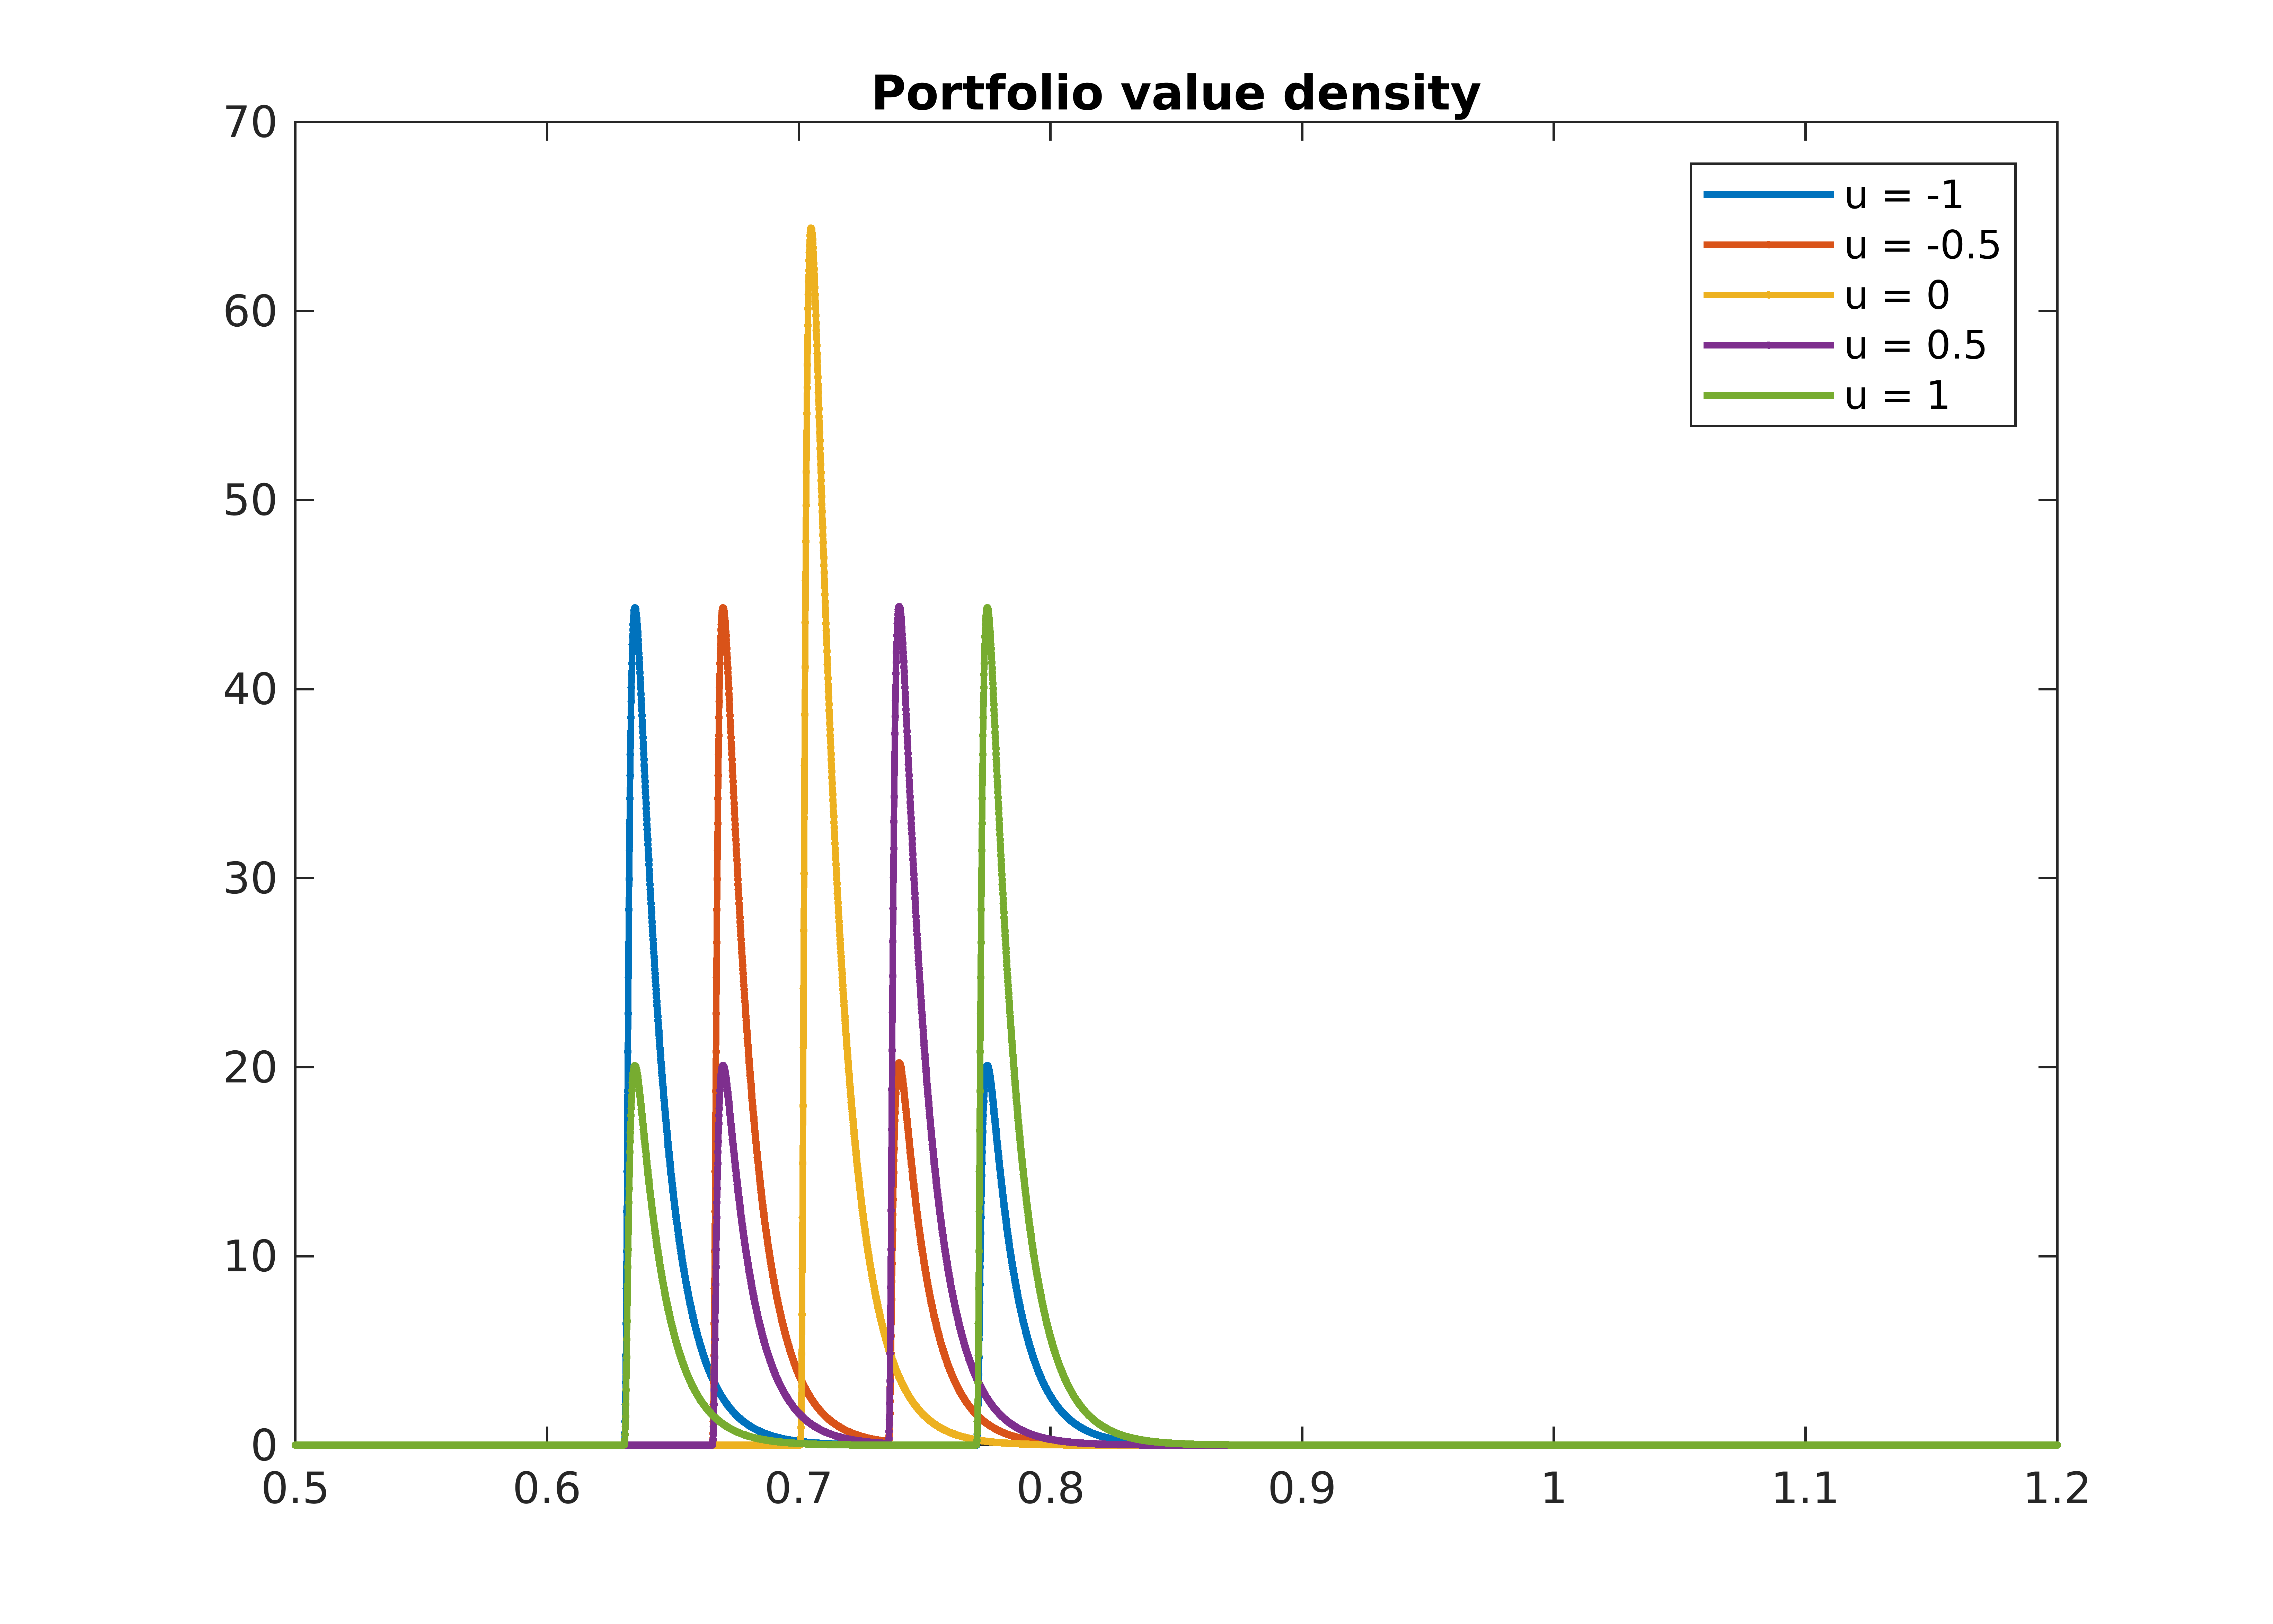
\includegraphics[scale = 0.5]{Images/PtfDensity}}
	\caption{Probability density function of random variable variable $x_{k+1}$ for different value of the risky-asset weight $u_k$ and the following parameters: $x=0.7$, $r=5.5\%$, $\mu=0.114$, $\sigma=0.1602$ and $J=10\%$}
	\label{fig:PtfDensity}
\end{figure}

\subsection{Numerical results}
In this section we report the results obtained by applying the \gls{ODAA} algorithm in an event-driven framework and modeling the risky asset as a Geometric Brownian Motion. Before showing the results however, we need to discuss the calibration of parameter $\mu$ and $\sigma$ of the \gls{GBM} dynamics to market data and the truncation of the series in (\ref{eq:Gamma}). As far as data is concerned, we use the same time series presented in Section \ref{sec:ED_dataset} (observations from the Future S\&P 500 index from 22 January 2010 to 25 April 2016).
\paragraph{\gls{GBM} calibration}
Let us consider the discretized solution of \gls{SDE} (\ref{eq:GBM_SDE})
\begin{align*}
S_{t_{k+1}} & = S_{t_k}\exp\big\{(\mu-\frac{1}{2}\sigma^2)\Delta t+\sigma(W_{t_{k+1}}-W_{t_k})\big\} \\
& = S_{t_k}\exp\big\{(\mu-\frac{1}{2}\sigma^2)\Delta t+\sigma\sqrt{\Delta t}Z\big\}
\end{align*}
where $Z \sim \mathcal{N}(0,1)$. In terms of log-return, we have
\[X_{t_{k+1}} = (\mu-\frac{1}{2}\sigma^2)\Delta t+\sigma\sqrt{\Delta t}Z.\] 
Let $x_1,\ldots,x_n$ be a random sample of log-returns from a normal population with mean $(\mu-\frac{1}{2}\sigma^2)\Delta t$ and variance $\sigma^2 \Delta t$. From this random sample we obtain the following estimates
\begin{align*}
\widehat{\sigma}^2 & = \frac{s^2}{\Delta t}\\[1.5ex]
\widehat{\mu} & = \frac{\bar{x}}{\Delta t} + \frac{1}{2}\widehat{\sigma}^2
\end{align*}
where $s^2$ is the sample variance and $\bar{x}$ the sample mean. Setting $\Delta t = 1/252$ and applying the equations above to our data we get $\widehat{\mu} = 0.0594$ and $\widehat{\sigma} = 0.1923$.


\paragraph{Series truncation}
In practice, the series in (\ref{eq:Gamma}) has to be truncated. Let $\Gamma^N_z(J)$ be the function in (\ref{eq:Gamma}) when the series is truncated at the $N$th term. The residual could be bounded in the following way
\begin{align*}
\big\lvert\Gamma^{\infty}_z(J)-\Gamma^N_z(J)\big\lvert & \leq \frac{\sigma^2\pi}{4J^2}\bigg\lvert\sum_{n=N+1}^{\infty}n(-1)^{n+1}z^{-\frac{1}{r}\big(\frac{\tilde{\mu}^2}{2\sigma^2} + \frac{\sigma^2n^2\pi^2}{8J^2}\big)-1}\sin(\frac{\pi}{2}n)\bigg\lvert\\
& \leq \frac{\sigma^2\pi}{4J^2} \sum_{n=N+1}^{\infty}nz^{-\frac{1}{r}\big(\frac{\tilde{\mu}^2}{2\sigma^2} + \frac{\sigma^2n^2\pi^2}{8J^2}\big)-1}\\
& \leq \frac{\sigma^2\pi}{4J^2} \int_{N}^{\infty}nz^{-\frac{1}{r}\big(\frac{\tilde{\mu}^2}{2\sigma^2} + \frac{\sigma^2n^2\pi^2}{8J^2}\big)-1}\mathrm{d}n\\
& \leq \frac{r}{\pi \log z}z^{-\frac{1}{r}\big(\frac{\tilde{\mu}^2}{2\sigma^2} + \frac{\sigma^2N^2\pi^2}{8J^2}\big)-1}
\end{align*}
therefore, denoting by $\epsilon$ the maximum error tolerance, we obtain
\begin{equation}
N(z) \geq \sqrt{-\frac{8rJ^2}{\sigma^2\pi^2}\bigg\{\frac{\widetilde{\mu}^2}{2r\sigma^2}+\log_z\Big(\frac{\epsilon\pi z \log z}{r}\Big) \bigg\}}.
\end{equation}
which is the minimum number of terms in the series in order to have the specified accuracy.

We considered an investment characterized by the following parameters:
\begin{itemize}
	\item Initial wealth $x_0 = 1$.
	\item $J = 10\%$.
	\item $N = 10$ portfolio rebalancings.
	\item The following target sets: $X_0 = \{1\}$, $X_k = [0,\infty)$ for $k = 1,\ldots,9$ and $X_{10} = [(1+\theta)^3,\infty)$  with $\theta=7\%$. In the implementation, they were approximated by $X_k = [0.5,1.9]$ for $k = 1,\ldots,9$ and $X_{10} = [(1+\theta)^3,1.9]$ and discretized with a step length of $5 \times 10^{-4}$.
	\item $r = 5.5\%$ (risk-free rate of return).
\end{itemize}
Some of the allocation maps obtained via \gls{ODAA} algorithm are reported in Figure \ref{fig:ext1_maps}. They exhibit the \textit{contatrian} attitude typical of all the \gls{ODAA} strategies presented so far. The joint probability of reaching the target sets is $p^{\star}=J(x_0) = 0.9727$. This result is verified by running a Monte Carlo simulation with $10^6$ replications at each rebalancing period, the outcome, in terms of joint probability and other investment statistics, is reported in Table \ref{tab:performance_ext1}. Finally, in Figure \ref{fig:ext1_investment_return} we show the empirical density function of the investment return.




\begin{figure}[H]
	%\centering
	\makebox[\textwidth][c]{
		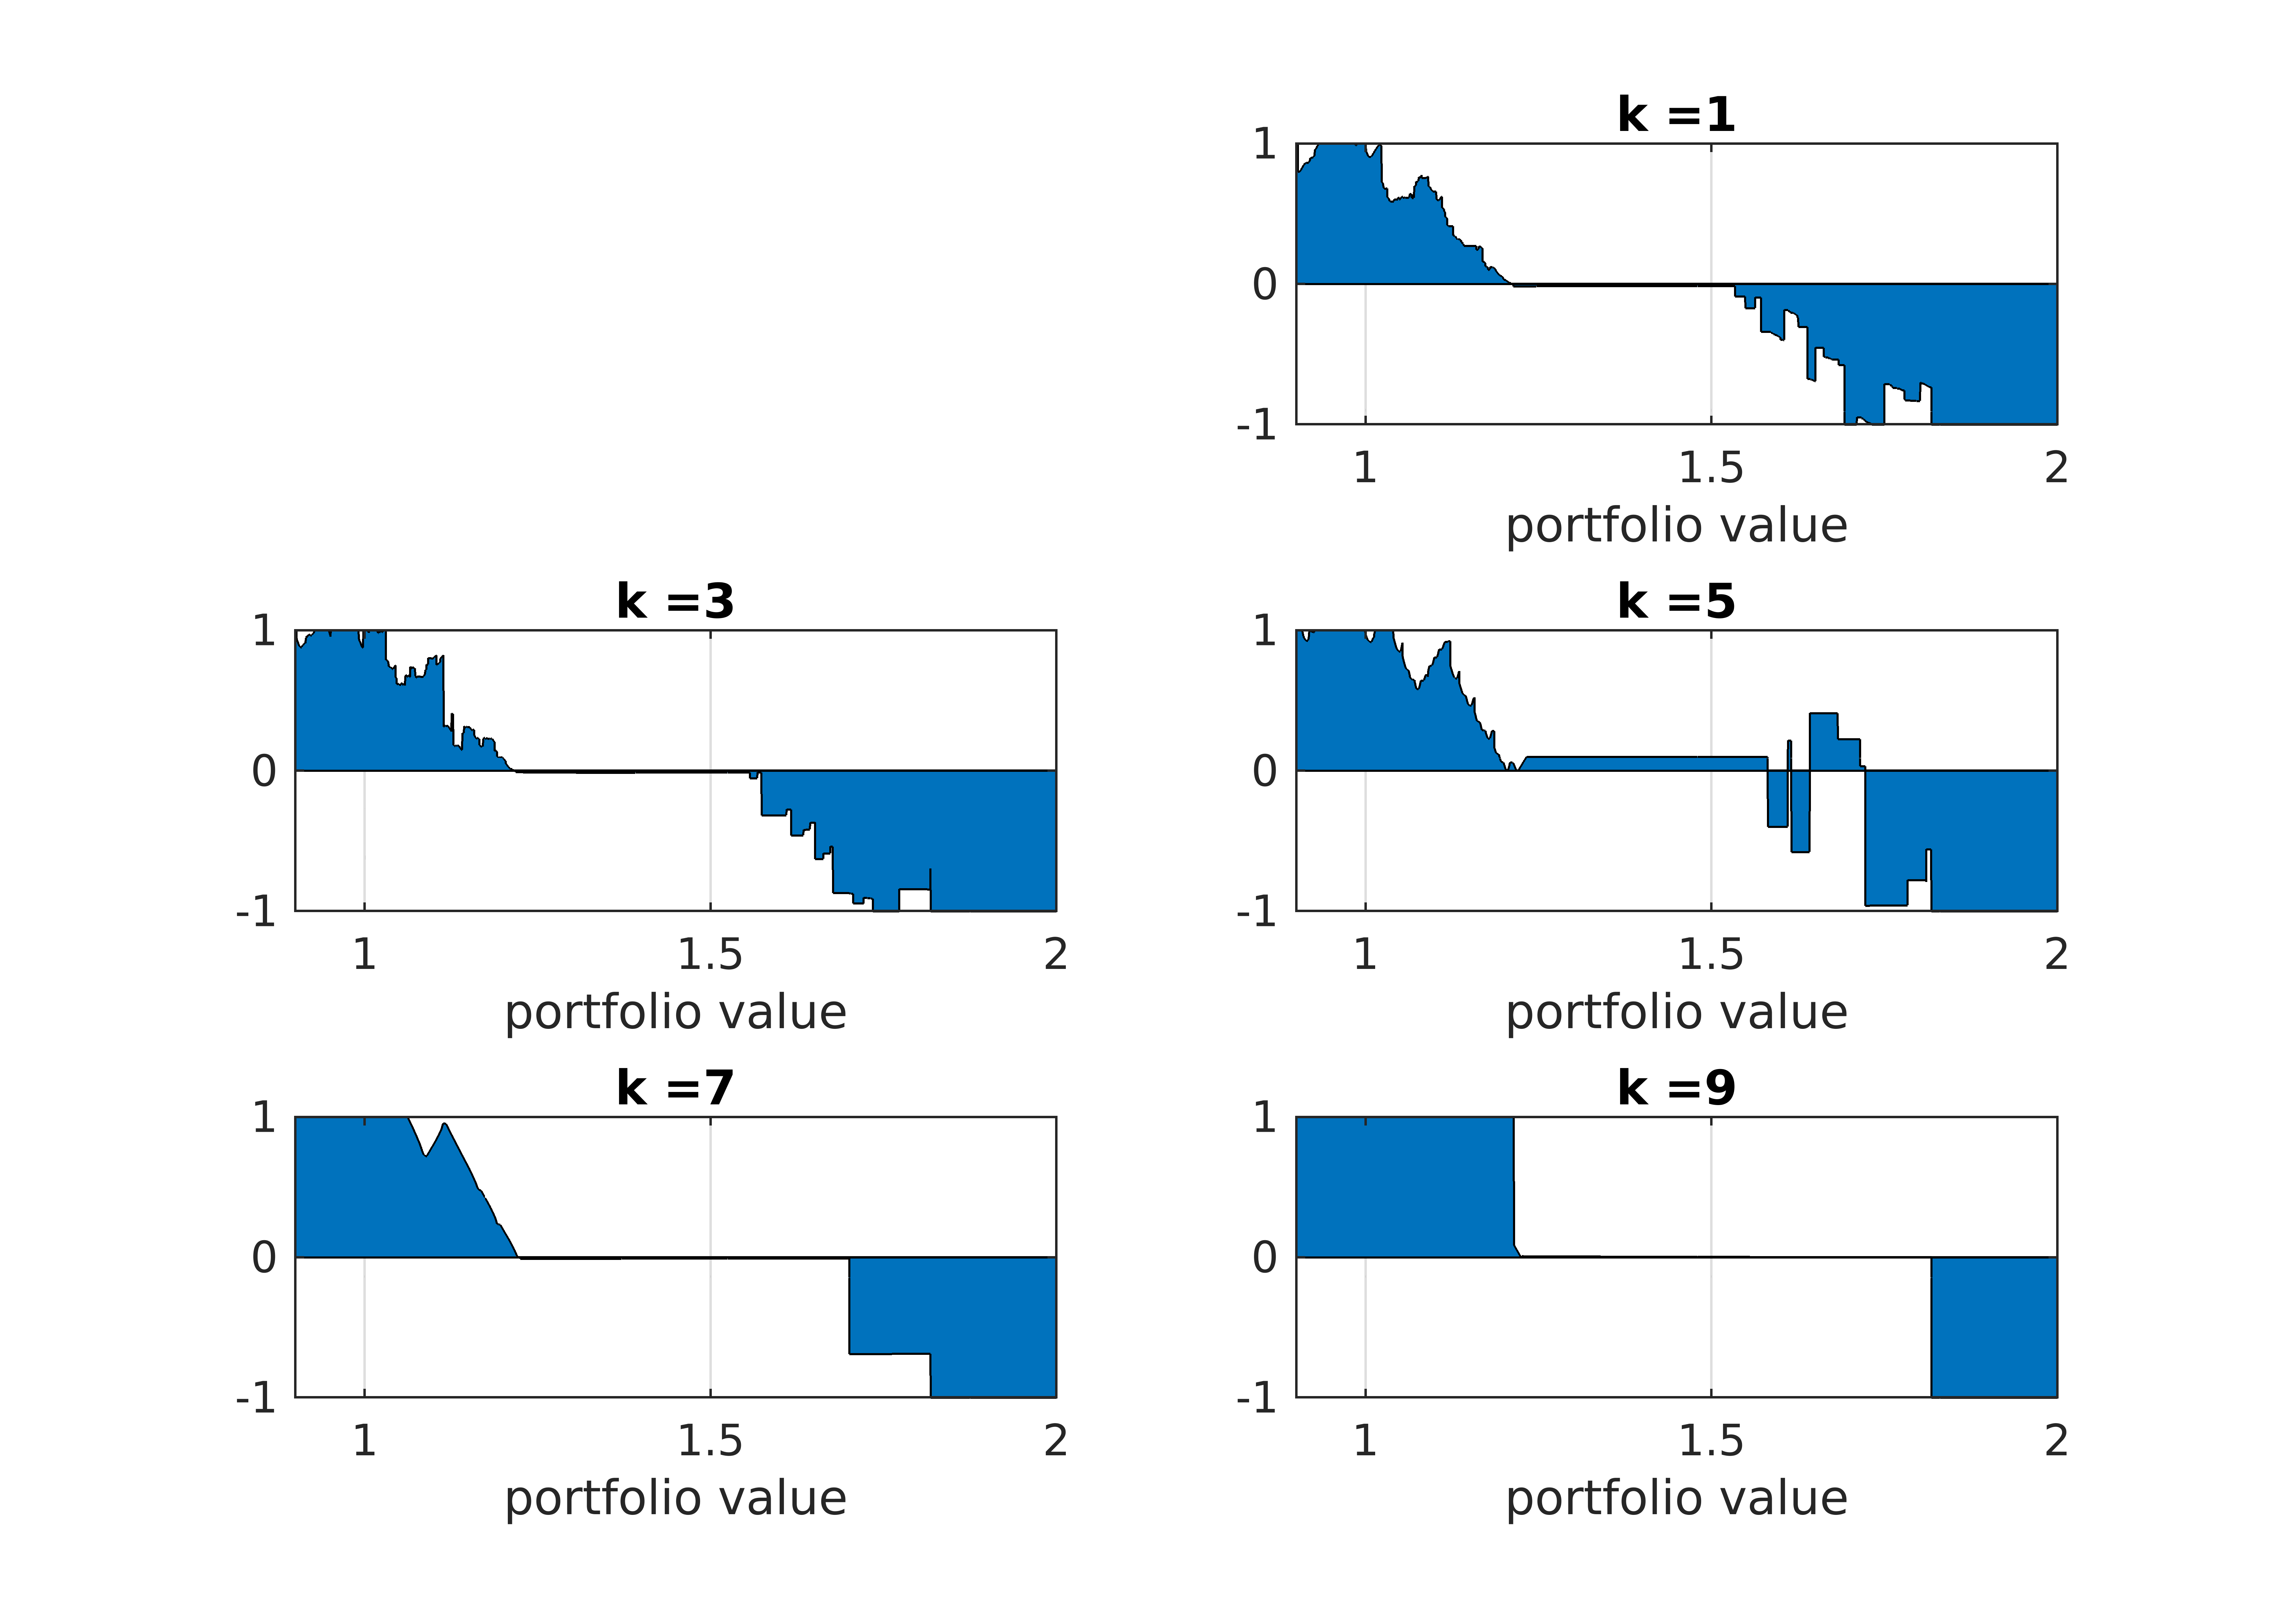
\includegraphics[scale = 0.8]{Images/mapsext1}}
	\caption{allocation maps for the risky asset, which is modeled according to a Geometric Brownian Motion }
	\label{fig:ext1_maps}
\end{figure}


\begin{figure}[H]
	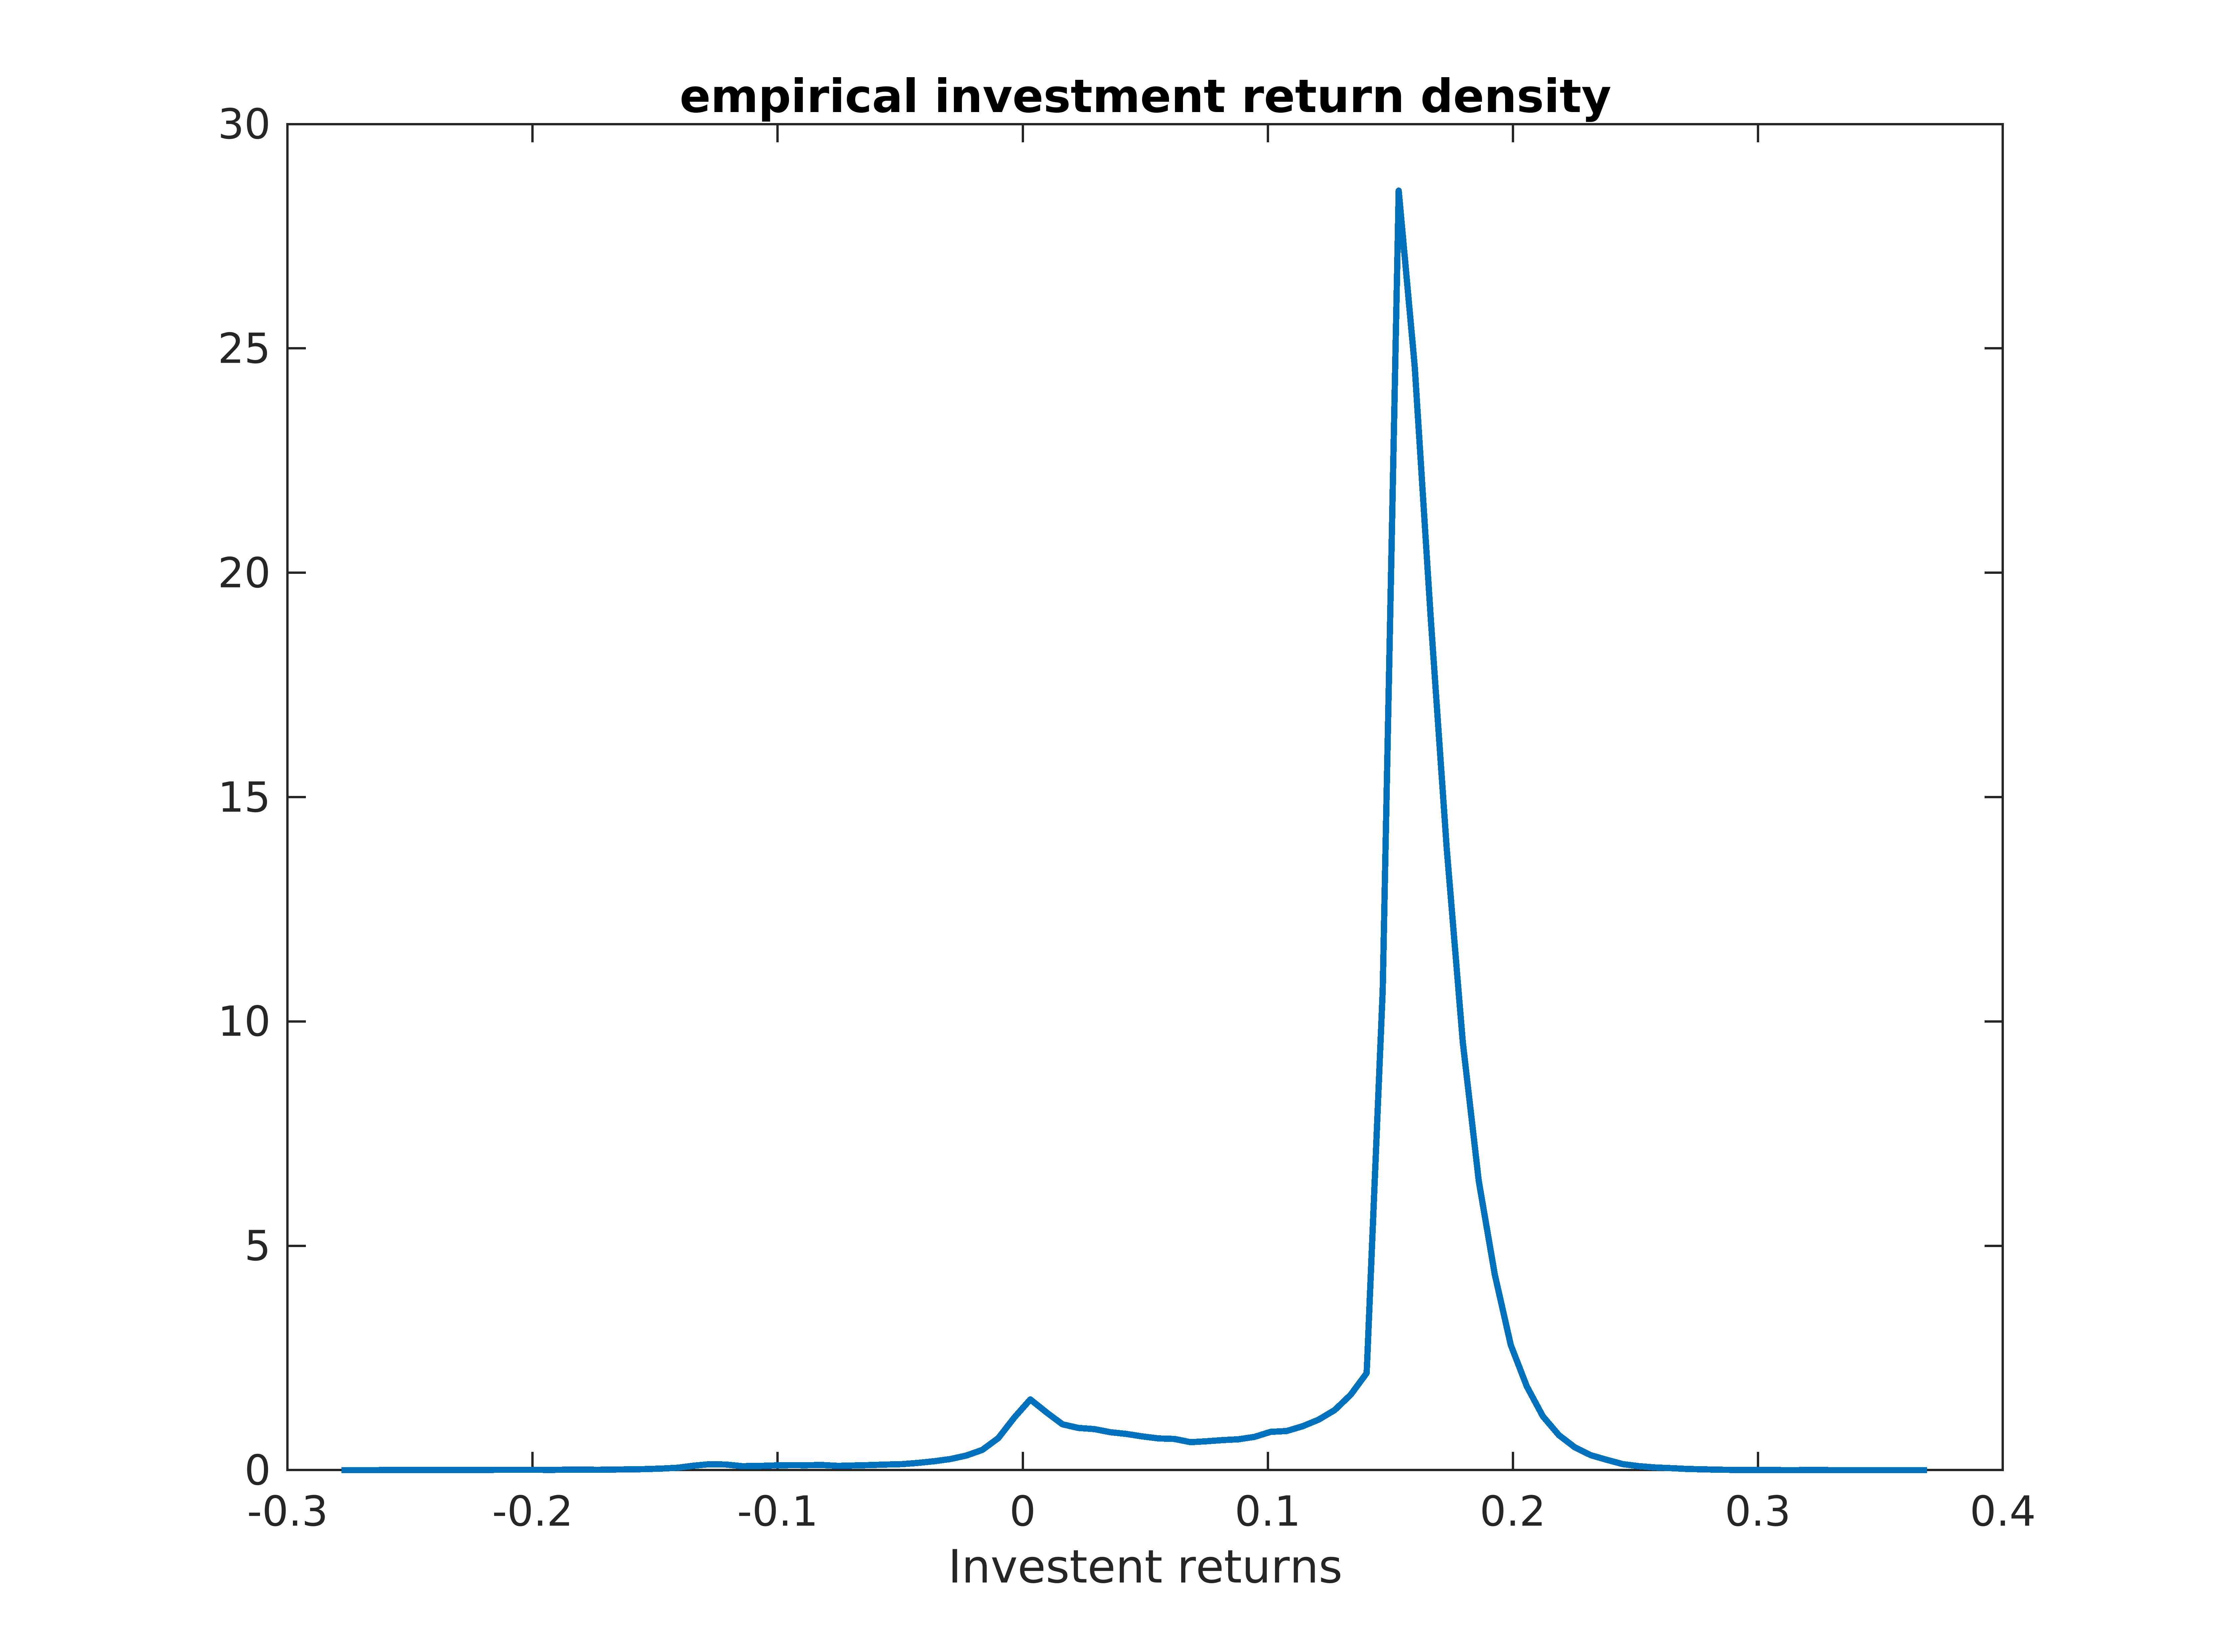
\includegraphics[scale = 0.4]{Images/Densityext1}
	\caption{Empirical density function of the investment return when the risky asset is modeled as a \gls{GBM}.}
	\label{fig:ext1_investment_return}
\end{figure}
\begin{wraptable}{l}{7cm}
		\begin{tabular}{@{}lc@{}}
			\toprule
			Statistics & value  \\
			%\addlinespace[0.5em]
			\midrule
			$p^{\star}$ & 0.9727\\
			\addlinespace[0.5em]	
			$p_{MC}$ & 0.9728\\
			\addlinespace[0.5em]
			Mean Return (ann) & 7.50\%\\
			\addlinespace[0.5em]
			Volatility (ann) & 3.93\%\\
			\addlinespace[0.5em]
			Median Return (ann) & 7.46\%\\
			\addlinespace[0.5em]
			Skewness & -1.81\\
			\addlinespace[0.5em]
			Kurtosis & 16.61\\
			\addlinespace[0.5em]
			Sharpe Ratio & 0.471\\
			\addlinespace[0.5em]
			Avg horizon [years] & 3.70 \\	
			\bottomrule
		\end{tabular}
		\caption{Investment performance obtained via Monte-Carlo simulation with $10^6$ replication at each rebalancing time.}
		\label{tab:performance_ext1}
\end{wraptable}

